\section{Our assigned user stories}\label{our-assigned-user-stories-sprint-2}
For sprint 2 we were assigned two user stories to implement.
In the following section we give a short introduction to Flutter and how we implemented the stories.

\subsection{Introduction to Flutter}
Flutter is built on the concept of widgets.
Widgets describe what their view should look like given their current configuration and state \cite{Flutterwidget}. 
They are classes to build UIs, used for both layout and UI elements.
Composing simple widgets lets you build complex widgets to create a layout \cite{Flutterlayout}.
Widgets typically extend either the \texttt{StatelessWidget} or \texttt{StatefulWidget} classes from the Flutter library.
\\\\
The difference is that \texttt{StatefulWidget} has the concept of a state within the widget, meaning it can change during the lifetime of the widget.
\texttt{StatefulWidgets} are used when part of the UI can change dynamically.
\texttt{StatelessWidgets} conversely do not have states, meaning they are useful when part of the UI does not depend on anything other than the basic information of the widget. 
Some of the basic widgets used to create a layout are \cite{FlutterBasicWidgets}:
 \begin{itemize}
    \item Container
    \item Row
    \item Column  
    \item Scaffold
    \item Text
    \item Image 
 \end{itemize} 
Most of these widgets are self explanatory. 
Rows let you layout a list of child widgets in the horizontal direction, columns let you do that in the vertical direction.
Container lets you customize its child widgets with, for example, margins or borders.
Scaffold helps structure the application, for example by determining where to place the top bar.

\subsection{The architecture of GIRAF}
The architecture of GIRAF is built on separate blocks to create functionality. 
The overall architecture is illustrated in \autoref{fig:architecture-giraf}.
\begin{figure}[h]
  \centering
  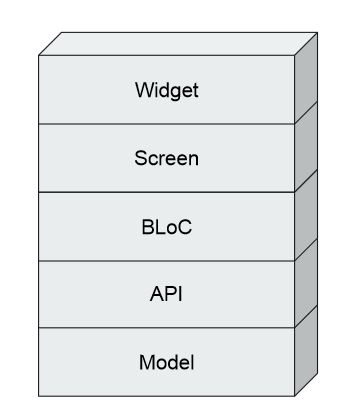
\includegraphics[width=0.3\textwidth]{girafarchitecture.JPG}
  \caption{The architecture of GIRAF}
  \label{fig:architecture-giraf}
\end{figure}
As shown in \autoref{fig:architecture-giraf}, the bottom layer is the \texttt{model}.
This layer is responsible for data, making sure what is required can be provided.
The next layer is the \texttt{API}, which is responsible for communication with the back end, to make sure that relevant data can be retrieved.
The \texttt{BLoC} layer is responsible for business logic. 
It uses streams and sinks to create states.
\begin{figure}[h]
  \centering
  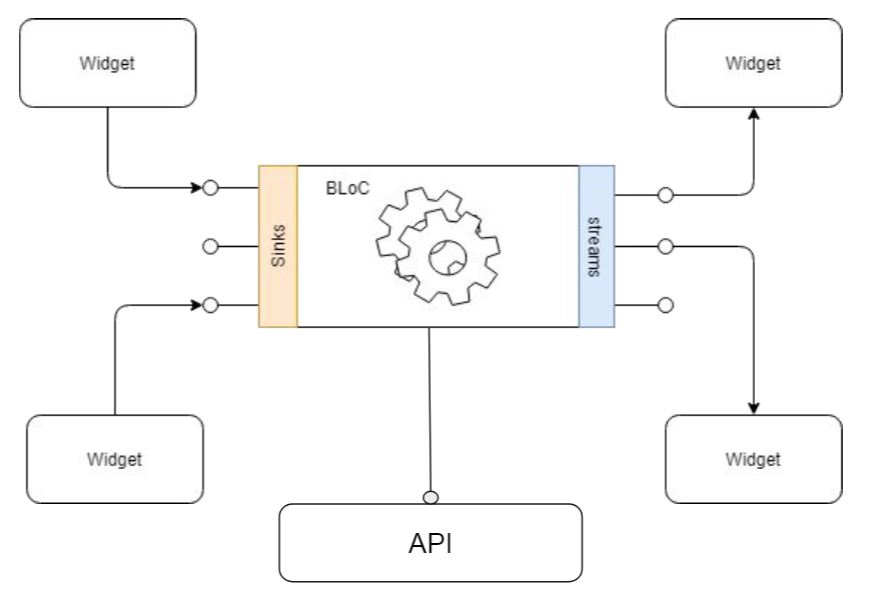
\includegraphics[width=0.6\textwidth]{streamsandsinks.JPG}
  \caption{A visual of streams and sinks}
  \label{fig:streamsandsinks}
\end{figure}
\noindent
As seen on \autoref{fig:streamsandsinks}, widgets send data to the \texttt{BLoC} through sinks, and streams send data from the \texttt{BLoC} to widgets.
This pattern is used to help ensure separation of responsibility, such that business logic can be changed without interfering with the application.  
Next is the \texttt{screen}, which is a page that can be visited, something that can be viewed.
Widgets are the final component.
These are smaller components that assist \texttt{screens} and help construct the actual layout of the page. 

\subsection{Our user stories and how we implemented them}
For sprint 2 we were assigned the following user stories:

\begin{itemize}
    \item "As a citizen I would like to be able to view my week plan so that I know what is going to happen"
    \item "As a guardian I would like to be able to view a given citizen's week plan so that I can get an overview of what is happening this week for them"
\end{itemize}
These user stories define essential functionality for the week planner - actually viewing the plan for both guardians and citizens.
This means we needed to implement the design for the basic view of the week planner, as defined by our prototypes.
The prototypes in \autoref{fig:story_weekplan_views} show the planned designs.

\begin{figure}[H]
  \begin{subfigure}{0.5\textwidth}
  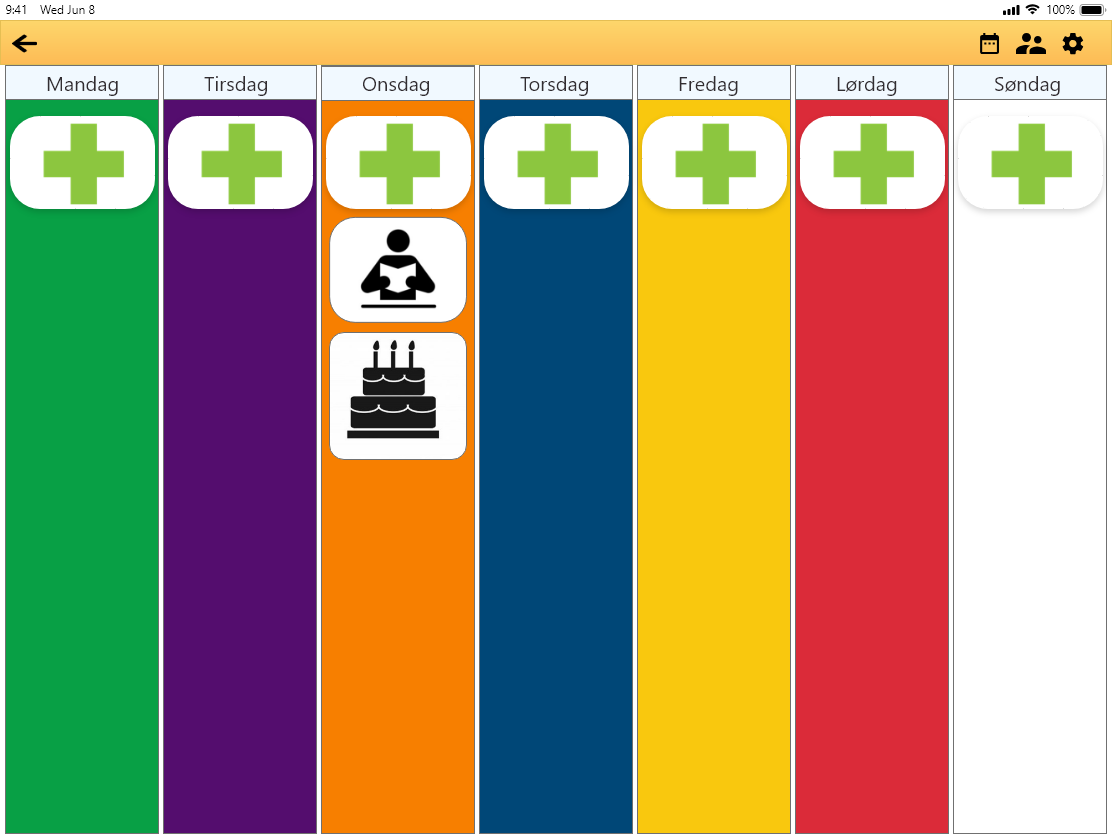
\includegraphics[width=1\linewidth, height=5cm]{ugeplan_guardian_view.png} 
  \caption{The guardian week plan}
  \label{fig:story_weekplan_guardian}
  \end{subfigure}
  \begin{subfigure}{0.5\textwidth}
      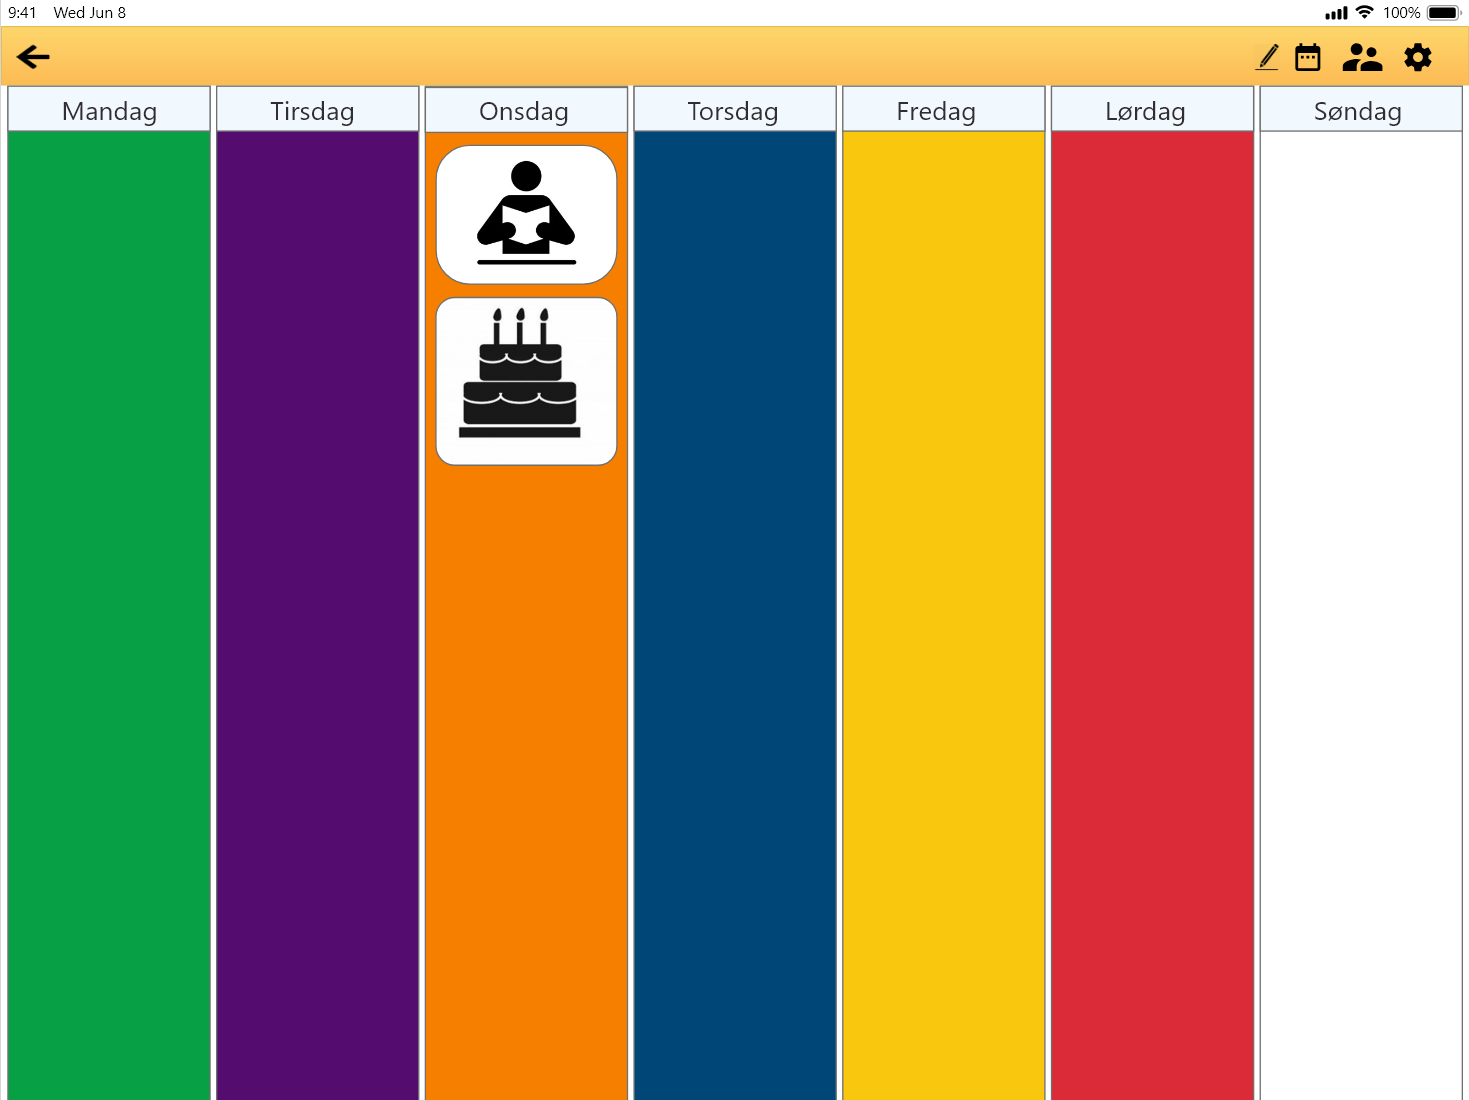
\includegraphics[width=1\linewidth, height=5cm]{weekplan_citizen_view.PNG}
  \caption{The citizen week plan}
  \label{fig:story_weekplan_citizen}
  \end{subfigure} 
  \caption{This figure shows both designs for the week plan.}
  \label{fig:story_weekplan_views}
\end{figure}

\subsubsection{The BLoC for the week plan view}
To implement the view the first thing needed is to implement the \texttt{BLoC} required, as this is the lowest level of the architecture that needs to be added for this functionality.

\begin{lstlisting}[caption={The week plan BLoC},label={lst:weekplanbloc}]
  class WeekplanBloc extends BlocBase {
    final Api _api;
    final BehaviorSubject<WeekModel> _week = BehaviorSubject<WeekModel>();

    WeekplanBloc(this._api);

    Stream<WeekModel> get week => _week.stream;

    void setWeek(WeekModel week) {
        _week.add(week);
    }

    @override
    void dispose() {
      _week.close();
    }
  }
\end{lstlisting}
The \texttt{WeekPlanBloc} class we implement extends the \texttt{BlocBase} abstract class.
This class acts as the base of all \texttt{BLoCs}, making sure they implement an override method.
At first we define an object of the \texttt{Api} class, which is used as a parameter for the constructor. 
We also instantiate a variable of the \texttt{WeekModel} class as a \texttt{BehaviorSubject}.
This means we instantiate a subject.
This subject has both a sink and a stream to control data.
Listeners can listen to the stream and be notified of updates.
As the subject is a \texttt{BehaviourSubject}, this means that, when subscribing to the stream, the listener is notified of the last event that happened on the stream prior to subscribing.
They are defined with the keyword \texttt{final} since they do not change values.
We instantiate the stream through the \texttt{week} variable.
The \texttt{setWeek} method creates the sink.


\subsubsection{The screen for the week plan view}
The \texttt{Screen} has to be implemented to give something for the user to view.
\begin{lstlisting}[caption={Setting up the screen},label={lst:screensetup}]
class WeekplanScreen extends StatelessWidget {
  final WeekplanBloc weekplanBloc = di.getDependency<WeekplanBloc>();

  WeekplanScreen({Key key, WeekModel week}) : super(key: key) {
    weekplanBloc.setWeek(week);
  }
  ...
\end{lstlisting}
\autoref{lst:screensetup} shows how the necessary dependencies for the screen are retrieved. 
It receives an instance of the \texttt{weekPlanBloc} through dependency injection.
The constructor takes a \texttt{Key} parameter, which is an identifier for widgets.
This key is received from the superclass.
The constructor also takes a \texttt{WeekModel} parameter, which is the definition of the week in the model component of the architecture. 
Finally it calls the \texttt{setWeek} method from the \texttt{BLoC} with the model for the week.

\begin{lstlisting}[caption={Building the structure},label={lst:screenstructure}]
  @override
  Widget build(BuildContext context) {
    return Scaffold(
      appBar: GirafAppBar(
        title: 'Ugeplan',
      ),
      body: StreamBuilder<WeekModel>(
        stream: weekplanBloc.week,
        initialData: null,
        builder: (BuildContext context, AsyncSnapshot<WeekModel> snapshot) {
          if (snapshot.hasData) {
            return _buildWeeks(snapshot.data);
          } else {
            return const Text('Data not ready');
          }
        },
      ),
    );
  }
\end{lstlisting}
\autoref{lst:screenstructure} shows how the overall structure of the screen is built. 
It returns a \texttt{Scaffold} that ensures the use of the GIRAF \texttt{AppBar}.
The \texttt{AppBar} is the bar at the top of most GIRAF screens that gives the user access to different functionalities.
It also defines the body of the scaffold, which is defined by a \texttt{StreamBuilder}.
The \texttt{StreamBuilder} is a widget that builds itself based on the latest interaction with a stream. 
The stream it builds is based on the \texttt{weekplanBloc.week} stream.
If the snapshot is not ready it just returns a \texttt{Text} message.

\begin{lstlisting}[caption={Building the week},label={lst:screenbuildweek}]
  Row _buildWeeks(WeekModel weekModel) {
  const List<int> weekColors = <int>[
    0xFF08A045,
    0xFF540D6E,
    0xFFF77F00,
    0xFF004777,
    0xFFF9C80E,
    0xFFDB2B39,
    0xFFFFFFFF
  ];
  final List<Widget> weekDays = <Widget>[];
  for (int i = 0; i < weekModel.days.length; i++) {
    weekDays.add(Expanded(
        child: Card(
            color: Color(weekColors[i]),
            child: _day(weekModel.days[i].day, weekModel.days[i].activities))));
  }
  return Row(children: weekDays);
}
\end{lstlisting}
\autoref{lst:screenbuildweek} builds the actual week on the screen.
At first, the colors are defined in hexadecimal, based on the colors defined in the design guide.
A list of widgets is instantiated, and a child is added for each day.
This child is of the widget type \texttt{Card}, which is the design used for a day.
These children are then returned as a \texttt{Row} widget, meaning that they are aligned horizontally.

\begin{lstlisting}[caption={Building days and activities},label={lst:screendaysandactivities}]
  Column _day(Weekday day, List<ActivityModel> activities) {
  return Column(
    children: <Widget>[
      _translateWeekDay(day),
      Expanded(
        child: ListView.builder(
          itemBuilder: (BuildContext context, int index) {
            return PictogramImage(
                //TODO: Redirect to show activity when it is implemented
                pictogram: activities[index].pictogram,
                onPressed: () => null);
          },
          itemCount: activities.length,
        ),
      ),
    ],
  );
  }
\end{lstlisting}
\autoref{lst:screendaysandactivities} shows how a day is built.
Days are of the \texttt{Column} widget class, meaning it is aligned vertically.
It takes a day as a parameter and a list of activities.
At first the name of the day is translated from English to Danish.
Then a \texttt{ListView} is created, which is a scrollable array. 
This is necessary since there can be a large amount of activities in a day, and the list of activities might exceed the size of the screen.
This \texttt{ListView} is populated by pictogram images based on the index of the activity.
When pressed, it should redirect to the detail page for this activity.
However, at the time of us completing this user story, the functionality to show detail for an activity was not implemented.


\subsubsection{The final design}
The design that was pushed to the develop branch of the GIRAF project at the end of the second sprint is shown in \autoref{fig:weekplanner_design}.
This design is used as the foundation for both the citizen mode and guardian mode views of the weekplanner.
The code in \autoref{lst:screenbuildweek} is responsible for the horizontal structure of the week, and the code from \autoref{lst:screendaysandactivities} is responsible for the vertical structure of single days.


\begin{figure}[H]
  \centering
  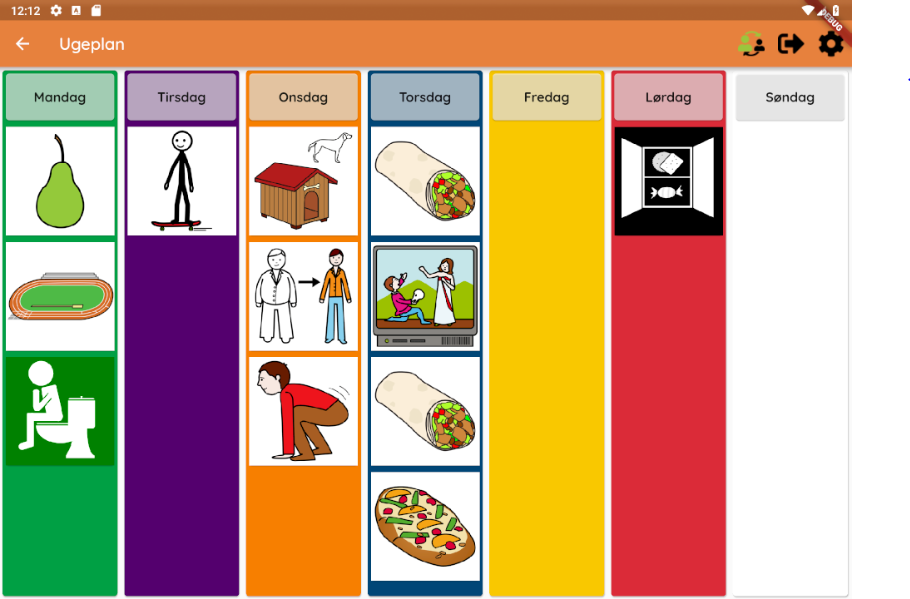
\includegraphics[width=0.5\textwidth]{ugeplan_view_implemented.PNG}
  \caption{The design of the weekplanner application as it was pushed to the master branch.}
  \label{fig:weekplanner_design}
\end{figure}